\chapter{Experiments\label{chap:experiments}}

\TODO{Rewrite when all included experiments are known.}
% Experiment setup and some signposting
We implemented  all variants and refinements of \algname{} described in \cref{chap:approach} in C++.
Our implementations of MSU3 and OLL were inspired by their implementations in Open-WBO~\autocite{DBLP:conf/sat/MartinsML14}, the other variants were implemented from scratch.
We used CaDiCaL~\autocite{BiereFazekasFleuryHeisinger-SAT-Competition-2020-solvers} as the internal SAT solver.
Additionally, we implemented $P$-minimal solution enumeration and Seesaw (see \cref{sec:sat-based}) as competing approaches, since no reference implementations were available.
As the hitting set solver for Seesaw, CPLEX 20.10 was used.
We evaluate the relative runtime performance of the \algname{} variants against the two competing approaches, as well as the impact of the specific refinements (recall \cref{sec:refinements}; employed as applicable, by default with heuristic core minimization and without blocking of dominated solutions) to \algname{} on their runtime performance.
As a parametric detail, in its default \msh{} is configured to switch between \msu{} and \satunsat{} once 70\% of the literals in $\Obj_\inc$ have been added to $\tot(\Act)$.
All experiments were run on 2.60-GHz Intel Xeon E5-2670 machines with 64-GB RAM in RHEL under a 1.5-hour per-instance time and 16-GB memory limit.

\section{Benchmarks\label{sec:benchmarks}}

% Signposting
We make use of two different benchmarking problems to empirically evaluate the performance of \algname{} and the competing approaches.
These two problems, learning interpretable decision rules from data and the bi-objective set covering problem, are described in the following two sections.

\subsection{Learning Interpretable Decision Rules\label{sec:lidr}}

% What is MLIC
Recently, a variety of SAT and MaxSAT-based approaches have been developed for learning interpretable classifiers from data~\autocite{DBLP:conf/ijcai/Ignatiev0NS21,DBLP:conf/cp/MaliotovM18,DBLP:conf/ijcai/NarodytskaIPM18,DBLP:conf/ijcai/Hu0HH20,DBLP:journals/corr/abs-2010-09919,DBLP:conf/cp/YuISB20,DBLP:conf/cade/IgnatievPNM18}.
The two objectives of minimizing size (the smaller, the more interpretable) and classification error (when there is no perfect classifier, as typical for real-world data) are conflicting, hence giving naturally rise to bi-objective optimization problems.
Here we consider learning of interpretable decision rules as a representative benchmark domain from this line of work, building on the encoding presented in~\textcite{DBLP:conf/cp/MaliotovM18}.
In short, here a decision rule is a binary classifier in the form of a CNF formula over boolean features.
The result of the formula evaluated on the features of a data sample is the classification assigned by the classifier to this sample.
In~\textcite{DBLP:conf/cp/MaliotovM18} a linear combination of the two objectives, using a parameter $\lambda\geq 0$, was proposed in order to directly apply a MaxSAT solver to find decision rules under a pre-fixed value for $\lambda$.
While this allows for finding a pareto-optimal decision rule under a specific value of $\lambda$, MaxSAT solving multiple times under different choices of $\lambda$ does not guarantee finding a representative pareto-optimal decision rule for each pareto point~\autocite{survey}.
In contrast, here we address directly the problem of computing all pareto-optimal solutions w.r.t.\ the two objectives.
\bigskip

% Example: Decision rule
\begin{minipage}{.75\textwidth}
  \begin{example}\label{ex:dr}
    Consider the sample dataset shown on the right with features $x_1$ and $x_2$, class $y$ and three samples.
    Two exemplary decision rules are the following: $r_1 = f_1$, $r_2 = f_1 \land f_2$.
    $r_1$ has size 1 and classification error 1 while $r_2$ has size 2 and classification error 0.
    Both $r_1$ and $r_2$ are pareto-optimal w.r.t\ size and classification error.
  \end{example}
\end{minipage}
\;
\begin{minipage}{.2\textwidth}
  \begin{center}
    \begin{tabular}{cc@{\hspace{2em}}c}
      \toprule
      $x_1$ & $x_2$ & $y$ \\
      \midrule
      1 & 1 & 1 \\
      0 & 1 & 0 \\
      1 & 0 & 0 \\
      \bottomrule
    \end{tabular}
  \end{center}
\end{minipage}
\bigskip

% The MLIC encoding and how we use it
For a gives set of $\nsamp$ data samples over $\nfeat$ features, the encoding uses two sets of variables:
$\selector_l^j$ for $l=1,\dots,\nclauses$, $j=1,\dots,\nfeat$ and $\noise_i$ for $i=1,\dots,\nsamp$ for a specific number $\nclauses$ of clauses in the decision rules to be learned, with the interpretation that $\selector_l^j=1$ iff the $j$th feature is included in the $l$th clause of the decision rule, and $\noise_i=1$ if the $i$th data sample is misclassified.
We represent the sample with index $i$ with a boolean class $y_i$ and the boolean features $x_i^j$ where $j=1,\dots,\nfeat$.
With this, the encoding is $\lnot \noise_i \rightarrow (y_i \leftrightarrow \bigwedge_{l=1}^\nclauses \bigvee_{j=1}^\nfeat (x_i^j \land \selector_l^j))$.
We use this encoding, literals $\selector_l^j$ as $\Obj_\inc$ and literals $\noise_i$ as $\Obj_\dec$.
This corresponds to finding pareto-optimal solutions w.r.t.\ the size of the decision rule as the total number of literals and its classification error.
We also consider swapping the objectives, so that the classification error is the increasing objective.

% Symmetry breaking clauses
Since decision rules in CNF contain many symmetric solutions obtained by changing the order of clauses, we add additional clauses to the encoding to break these symmetries.
The idea behind the symmetry breaking is that the bit-strings $\sol(\selector_l^1)\sol(\selector_l^2)\dots\sol(\selector_l^\nfeat)$ are forced to be in lexicographic ordering.
In addition to the $\selector$ variables, we introduce variables $\equals_l^j$ for $j=1,\dots,\nfeat$ and $l=2,\dots,\nclauses$ that represent whether the bit-strings of the clauses with index $(l-1)$ and $l$ are equal for the first $j$ bits.
The semantics of this representation are encoded as follows:
$\equals_l^1 \leftrightarrow (\selector_{l-1}^1 \leftrightarrow \selector_l^1)$ and $\equals_l^j \leftrightarrow (\equals_l^{j-1} \land (\selector_{l-1}^f \leftrightarrow \selector_l^j))$ for $j=2,\dots,\nfeat$.
The lexicographic ordering is then enforced by adding the constraints $\lnot \equals_l^1 \rightarrow (\selector_{l-1}^1 \land \lnot \selector_{l-1}^1)$ and $(\equals_l^{j-1} \land \lnot \equals_l^j) \rightarrow (\selector_{l-1}^j \land \lnot \selector_l^j)$ for $j=2,\dots,\nfeat$, enforcing that the bit with the smallest index in which the clauses differ should be 1 in the clause with index $(l-1)$ and 0 in the clause with index $l$.

% Example: Symmetric decision rules
\begin{example}
  Consider the rule $r_2 = f_1 \land f_2$ for the data in \cref{ex:dr}.
  It consists of two clauses, $C_1 = f_1$ and $C_2 = f_2$.
  In a solution $\sol$ to the encoding, $C_1$ will be represented as the bit-string $\sol(\selector_l^1)\sol(\selector_l^2)=10$ and $C_2$ as $\sol(\selector_l^1)\sol(\selector_l^2)=01$.
  Without symmetry breaking, either $\sol_1 = \{\selector_1^1, \lnot\selector_1^2, \lnot\selector_2^1, \selector_2^2\}$ or $\sol_2 = \{\lnot\selector_1^1, \selector_1^2, \selector_2^1, \lnot\selector_2^2\}$ would be valid solutions, even though they both map to $r_2$.
  The symmetry breaking clauses enforce that the bit-string representing $C_1$ precedes the bit-string representing $C_2$, therefore only $\sol_1$ is a feasible solution.
\end{example}

% Benchmark datasets
As the basis of our benchmark instances, we used 24 standard UCI~\autocite{UciMlr} and Kaggle ({\small\url{https://www.kaggle.com}}) benchmark datasets, including ones used in~\textcite{DBLP:conf/cp/MaliotovM18}; see \cref{appendix:datasets} for details.
We randomly and independently sampled subsets of $\nsamp\in\{50,100,1000,5000,10000\}$ data samples from the datasets, four of each size (when applicable), resulting in a total of 372 datasets.
The datasets were discretized as in~\textcite{DBLP:conf/cp/MaliotovM18}:
categorical features are one-hot encoded, continuous features discretized by comparing to a collection of thresholds.
All experiments on these datasets were run with the encoding from~\textcite{DBLP:conf/cp/MaliotovM18} configured to learn CNF decision rules consisting of two clauses.

% domain-specific blocking
When enumerating multiple solutions corresponding to the same pareto point, the blocking clauses for \algname{} (as well as the $P$-minimal approach compared to in the experiments) can be strengthened to find solutions mapping to distinct rules:
blocking over the variables $s_l^j$ is sufficient and blocks multiple symmetric solutions that only differ in the assignment to auxiliary variables.
Further, making use of the algorithm-specific fact that \algname{} is guaranteed to enumerate pareto-optimal solutions in order of increasing size, for \algname{} it is sufficient to block a solution over all $s_l^j$ that are assigned to false.

% Seesaw instantiation for MLIC
We instantiated Seesaw for learning interpretable decision rules by using misclassifications as the objective over which cores are extracted and a hitting set $\hs$ is found over these cores.
In the second step, the number of literals in the smallest rule misclassifying the samples in $\hs$ or a subset of it is found.
This function is implemented as a solution-improving search with a SAT solver.
This instantiation was chosen because finding the smallest rule misclassifying $\hs$ is an anti-monotone function and the refined version of core extraction presented in~\textcite{DBLP:conf/cp/JanotaMSM21} can therefore be used, making Seesaw feasible in the first place.

\subsection{Bi-Objective Set Covering}

% Bi-objective set covering and its encoding
In the set covering problem over sets $\sets$, a subset $\cover$ of the elements $\{1,\dots,\nelems\}$ needs to be chosen such that (i)~$\cover$ covers all sets in $\sets$, i.e., $\cover\cap S\neq\emptyset,\,\forall S\in\sets$, and (ii)~$\cover$ is minimal regarding some objective.
The bi-objective variant assigns each element $\element$ two different cost values $\cost^\element_1$ and $\cost^\element_2$ where the two different objectives for the cover $\cover$ are to minimize $c^\cover_1 = \sum_{\element\in\cover}\cost^\element_1$ and $c^\cover_2 = \sum_{\element\in\cover}\cost^\element_2$.
When encoding set covering into propositional logic, every set $S\in\sets$ forms one clause in the encoding, i.e., the clauses are $\{l_\element \mid \element\in S\}$ with $l_\element$ being a literal representing if element $\element$ is in $\cover$.
Furthermore, the integer values for the cost associated with element $\element$ can be represented by adding $l_\element$ to the objective set $\cost^\element$ times.
Note that multi-objective set covering was also used originally for evaluating $P$-minimal~\autocite{DBLP:conf/cp/SohBTB17}.

% Example: Set covering
\begin{example}
  Consider the sets $\sets = \{ \{a, b\}, \{b, d\} \}$ and costs $c^a_1 = c^b_1 = c^d_1 = c^a_2 = c^d_2 = 1$ and $c^b_2 = 5$.
  The two covers $\cover_1 = \{ b \}$ and $\cover_2 = \{ a, b \}$ are pareto-optimal with $\cover_1$ having costs $c^{\cover_1}_1 = 1$ and $c^{\cover_1}_2 = 5$ and $\cover_2$ costs $c^{\cover_2}_1 = 2$ and $c^{\cover_2}_2 = 2$.
\end{example}

% Benchmark instances
We generated two types of  bi-objective set covering problem instances:
(i)~using a fixed probability $\elemprob$ for an element appearing in a set (\scep{}), and (ii)~using fixed set cardinality $\setcard$, with elements in a set chosen uniformly at random without replacement (\scsc{}).
We generated both types of instances using combinations of the following parameters:
number of elements $\nelems\in\{100,150,200\}$, number of sets $\nsets\in\{20,40,60,80\}$, element probability $\elemprob\in\{0.1,0.2\}$ and set cardinality $\setcard\in\{5,10\}$.
For each combination, we generated five instances, leading to 120 instances of each type.
The integer cost values $\cost$ for the two objectives were chosen uniformly at random from the range $\cost\in[1,100]$.

% Domain-specific blocking
The blocking clauses used in \algname{} for enumerating all pareto-optimal solutions can be strengthened also for set covering:
due to the fact that \algname{} is guaranteed to enumerate the pareto-optimal solutions so that one of the objectives will monotonically decrease, it is enough to block in \algname{} the solution over all $l_e$ that are assigned to true.

% Seesaw not feasible
Since both objectives in the bi-objective set covering problem are monotone over the chosen cover, the refined core extraction strategy for Seesaw from~\textcite{DBLP:conf/cp/JanotaMSM21} cannot be used.
Seesaw is therefore infeasible for this problem since it would enumerate every possible solution.

\section{Results\label{sec:results}}

% Signposting
In this section, we present the results of the experiments we performed.
We start with a performance comparison of the different approaches for the task of finding a single representative solution per pareto point.
Following that, we do the same comparison for the task of finding all pareto-optimal solutions.
In the last subsection, we look at how the different refinements presented in \cref{sec:refinements} influence the performance of \algname{}.

\subsection{Finding a Single Representative Solution per Pareto Point}

% mlic-cactus-single
For comparing the performance of the variants of \algname{} presented in \cref{sec:variants}, $P$-minimal and Seesaw, we first look at the results for learning a single decision rule per pareto point.
\Cref{fig:mlic-cactus-single} shows the number of instances solved ($x$-axis) for different per-instance time limits ($y$-axis) for this task.
The best-performing approach is the \algname{} variant \msh{}, solving 223 instances, while $P$-minimal solved 219 instances.
All variants of \algname{} outperform $P$-minimal to some extent.
Seesaw is very clearly outperformed by all other approaches, solving only 123 instances within the resource constraints.

% mlic-cactus-single
\begin{figure}
    \centering
    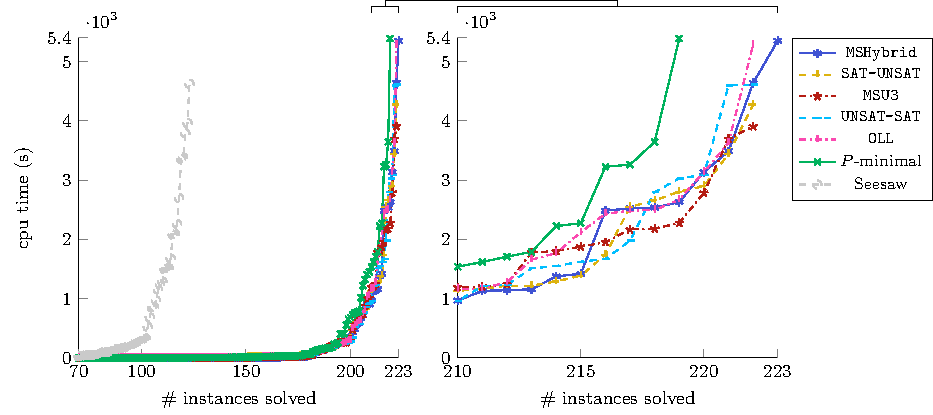
\includegraphics{mlic-cactus-single.pdf}
    \caption{Runtime comparison of $P$-minimal and variants of \algname{} for learning interpretable decision rules;
      enumeration of a single representative solution per pareto point.
      Plot on the right is zoomed in on the more interesting part of the left plot.
    }\label{fig:mlic-cactus-single}
\end{figure}

% setcover-cactus-single
Next we look at a similar comparison for the bi-objective set covering benchmarks.
In this comparison, Seesaw is not included since it cannot be feasibly instantiated for this task.
\Cref{fig:setcover-cactus-single} shows the number of solved instances per individual time limit for the two generated sets of bi-objective set covering instances.
Here again \msh{} is the best-performing variant of \algname{}, considerably outperforming $P$-minimal:
$P$-minimal solved 71 (respectively 38) fixed element probability (respectively set cardinality) instances, whereas \msh{} solved 82 (respectively 40) instances.
For this application, not all variants of \algname{} outperformed $P$-minimal:
\msu{} and \oll{} were outperformed for both instance variants while \satunsat{} and \unsatsat{} were only outperformed for the instances generated with fixed set cardinality.

% setcover-cactus-single
\begin{figure}
    \centering
    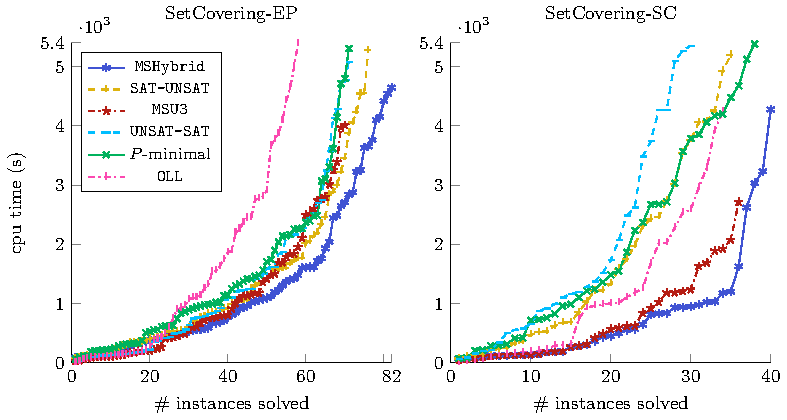
\includegraphics{setcover-cactus-single.pdf}
    \caption{Runtime comparison of $P$-minimal and variants of \algname{} for bi-objective set covering problem;
      enumeration of a single representative solution per pareto point.
    }\label{fig:setcover-cactus-single}
\end{figure}

% Overall solved instances and best-performaning
The numbers of solved instances for all approaches (except Seesaw) are summarized in \cref{tab:nsolved-single}.
The best-performing approach for each benchmark is highlighted in bold font.
\msh{} is the best-performing \algname{} variant overall, outperforming $P$-minimal in all cases.
For more details, \cref{fig:msh-scatter-single} shows a per-instance runtime comparison between \msh{} and $P$-minimal.
We note that $P$-minimal did not uniquely solve any instance.
In general, \msh{} was outperformed by $P$-minimal on only 37 instances while \msh{} solved 308 instances in less time.

% nsolved-single
\begin{table}
  \centering
  \caption{Solved instances by approach and benchmark family;
    enumeration of a single representative per pareto point.
  }\label{tab:nsolved-single}
  \begin{tabular}{@{}lrrrrrr@{}}
    \toprule
    Instance Type & \satunsat{} & \unsatsat{} & \msu{} & \oll{} & \msh{} & $P$-minimal \\
    \midrule
    Decision Rules & 222 & 222 & 222 & 222 & \textbf{223} & 219 \\
    \scep{} & 76 & 71 & 70 & 58 & \textbf{82} & 71 \\
    \scsc{} & 35 & 30 & 36 & 34 & \textbf{40} & 38 \\
    \bottomrule
  \end{tabular}
\end{table}

% msh-scatter-single
\begin{figure}
  \centering
  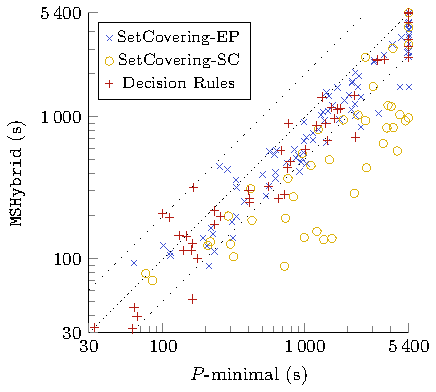
\includegraphics{all-datasets-msh-scatter-log-single.pdf}
  \caption{Runtime comparison between $P$-minimal and \algname{} in the \msh{} variant;
    enumeration of a single representative per pareto point.
  }\label{fig:msh-scatter-single}
\end{figure}

\subsection{Enumerating All Pareto-Optimal Solutions}

% mlic-cactus-multi
Next we compare the performance for learning all pareto-optimal interpretable decision rules.
\Cref{fig:mlic-cactus-multi} shows the results for this task, presented in the same way as in \cref{fig:mlic-cactus-single}.
For this task, the \algname{} variants \satunsat{}, \unsatsat{}, \msu{} and \msh{} all performed the best, solving 215 instances each.
With this, they outperform $P$-minimal, which only solved 213 instances.
For this task, the \oll{} variant of \algname{} does not manage to outperform $P$-minimal.
Note that the Seesaw configuration included in \cref{fig:mlic-cactus-multi} does not strictly solve the same task as the other.
As mentioned previously, Seesaw cannot be easily extended to enumerate all pareto-optimal solutions, we still include it here to show that even when solving the potentially more complex task of enumerating all pareto-optimal solutions, the other approaches clearly outperform Seesaw.

% mlic-cactus-multi
\begin{figure}
  \centering
  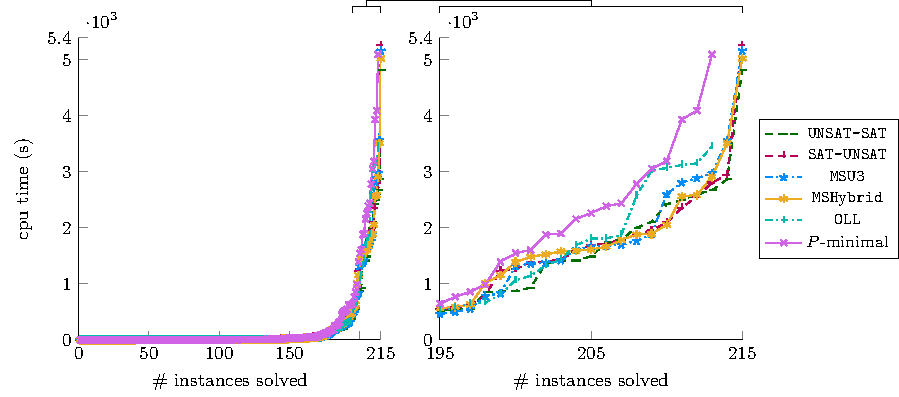
\includegraphics{mlic-cactus.pdf}
  \caption{Runtime comparison of  $P$-minimal and variants of \algname{} for learning interpretable decision rules;
    enumeration of all pareto-optimal solutions.
    Plot on the right is zoomed in on the more interesting part of the left plot.
  }\label{fig:mlic-cactus-multi}
\end{figure}

% setcover-cactus-multi
Looking at the same comparison for bi-objective set covering, we can see in \cref{fig:setcover-cactus-multi} that \msh{} was the best-performing approach also here.
For the instances with fixed set cardinality, all \algname{} variants solved at least as many instances as $P$-minimal, for the instances with fixed element probability only \oll{} was outperformed.
The best-performing variant, \msh{}, solved 80 (respectively 40) of the fixed element probability (respectively set cardinality) instances while $P$-minimal only solved 68 (respectively 26).

% setcover-cactus-multi
\begin{figure}
  \centering
  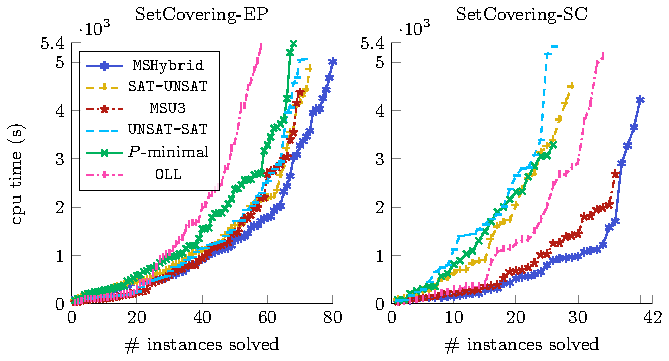
\includegraphics{setcover-cactus.pdf}
  \caption{Runtime comparison of $P$-minimal and variants of \algname{} for bi-objective set covering problem;
    enumeration of all pareto-optimal solutions.
  }\label{fig:setcover-cactus-multi}
\end{figure}

% Overall solved instances and best-performing
\Cref{tab:nsolved-multi} summarizes the number of solved instances for all approaches applicable to this task.
The best-performing approach for each benchmark is highlighted in bold font.
It can be seen that \msh{} is the best-performing approach for this task as well.
A per-instance runtime comparison between \msh{} and $P$-minimal for the task of enumerating all pareto-optimal solutions can be seen in \cref{fig:combined-msh-scatter-single-multi} (left).
$P$-minimal did also not uniquely solve any instance for enumerating all pareto-optimal solutions.
Furthermore, \msh{} was outperformed by $P$-minimal on 69 instances while \msh{} solved 256 instances faster.

% nsolved-multi
\begin{table}
  \centering
  \caption{Solved instances by approach and benchmark family;
    enumeration of all pareto-optimal solutions.
  }\label{tab:nsolved-multi}
  \begin{tabular}{@{}lrrrrrr@{}}
    \toprule
    Instance Type & \satunsat{} & \unsatsat{} & \msu{} & \oll{} & \msh{} & $P$-minimal \\
    \midrule
    Decision Rules & \textbf{215} & \textbf{215} & \textbf{215} & 212 & \textbf{215} & 213 \\
    \scep{} & 73 & 71 & 70 & 58 & \textbf{80} & 68 \\
    \scsc{} & 29 & 26 & 36 & 34 & \textbf{40} & 26 \\
    \bottomrule
  \end{tabular}
\end{table}

% Single multi comparison
Comparing the number of solved instances between \cref{tab:nsolved-single} and \cref{tab:nsolved-multi}, we can see that the performance difference between \algname{} and $P$-minimal is greater when enumerating all pareto-optimal solutions.
Furthermore, \cref{fig:combined-msh-scatter-single-multi} (right) shows a runtime comparison between enumerating a single representative solution per pareto point and enumerating all pareto-optimal solutions with \msh{}.
Overall, the approach scales well also for the latter task, although there understandable is an overhead when the number of solutions required to be enumerated grows significantly;
this is the case for learning interpretable decision rules, where some instances have more than 10\,000 solutions per pareto point.
This is in contrast to the set covering instances, which tend to have only a single (of few) solutions per pareto point.
The fewer solutions per pareto point for the set covering instances can be explained by the weighted objectives which make it significantly less likely that two distinct solutions have identical objective function values.

% combined-msh-scatter-single-multi
\begin{figure}
  \centering
  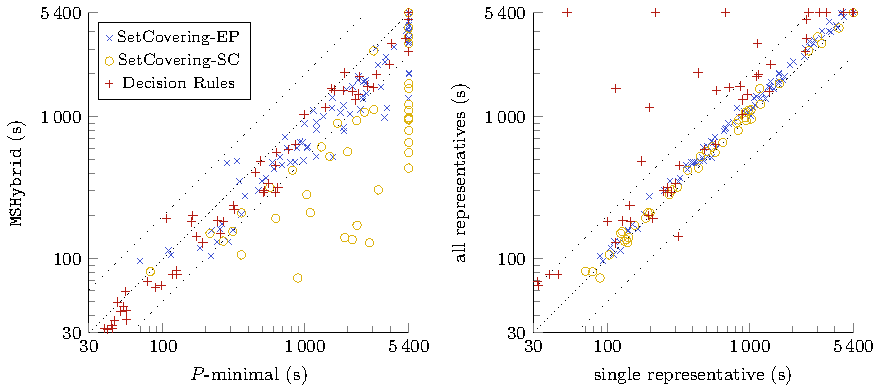
\includegraphics{all-datasets-combined-msh-and-enumeration.pdf}
  \caption{Left: Runtime comparison between $P$-minimal and \algname{} in the \msh{} variant; 
    enumeration of all pareto-optimal solutions.
    Right: Runtime comparison between enumerating a single representative vs.\ all solutions per pareto point with \msh{}.}\label{fig:combined-msh-scatter-single-multi}
\end{figure}

\subsection{Impact of Refinements}

% Lazily building the totalizer for the decreasing objective
Finally, we evaluated the impact of the refinements proposed in \cref{sec:refinements} on the runtime efficiency of the best-performing approach, \msh{}.
As the first refinement considered, we evaluate the impact of lazily building the totalizer for the decreasing objective.
\Cref{fig:refinements-1} (left) shows a runtime comparison between \msh{} with and without lazy building of $\tot(\Obj_\dec)$.
It can be seen that for learning interpretable decision rules, this refinement has no evident impact.
This is to be expected since the for these benchmarks, the literals from $\Obj_\dec$ do not appear in $\Obj_\inc$, so $\tot(\Obj_\dec)$ cannot be lazily built.
For the set covering instances with fixed element probability, the impact of this refinement is small and tends to be slightly negative for most instances.
For fixed set cardinality set covering however, we see a strong positive effect.

% Core minimization
Next, we look at the impact of different core minimization strategies.
By default, \msh{} employs heuristic core minimization, in \cref{fig:refinements-1} (right), the performance of this configuration is compared to using exact core minimization instead.
Heuristic core minimization appears to have a positive effect for the task of learning interpretable decision rules as well as for harder set covering instances.
However, the differences to exact minimization are smaller than those regarding lazily building $\tot(\Obj_\dec)$.

% refinements-1
\begin{figure}
    \centering
    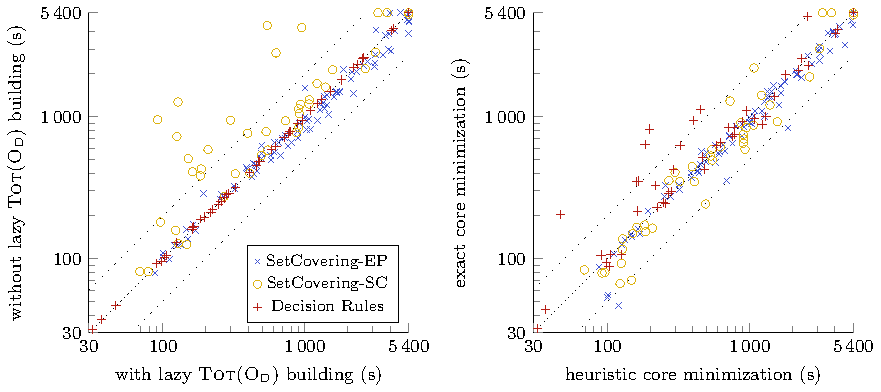
\includegraphics{all-datasets-chosen-refinements-1.pdf}
    \caption{Instance runtime comparisons for the two refinements lazily building the totalizer for the decreasing objective (left) and exact core minimization (right).}\label{fig:refinements-1}
\end{figure}

% Blocking dominated solutions
\Cref{fig:refinements-2} (left) shows the effect of adding the blocking of dominated solutions in the \satunsat{} phase of \msh{}.
The impact of this refinement is miniscule on all benchmarks.

% Disjoint phase
As the last refinement considered, we look at adding a disjoint phase to the \msu{} phase of \msh{}.
\Cref{fig:refinements-2} shows the impact of adding this refinement to the default configuration of \msh{}.
It can be seen that the impact on the set covering instances is fairly small but slightly positive.
In contrast to that, the impact on the instances for learning interpretable decision rules is overall negative and slightly stronger than for the set covering instances.

% refinements-2
\begin{figure}
    \centering
    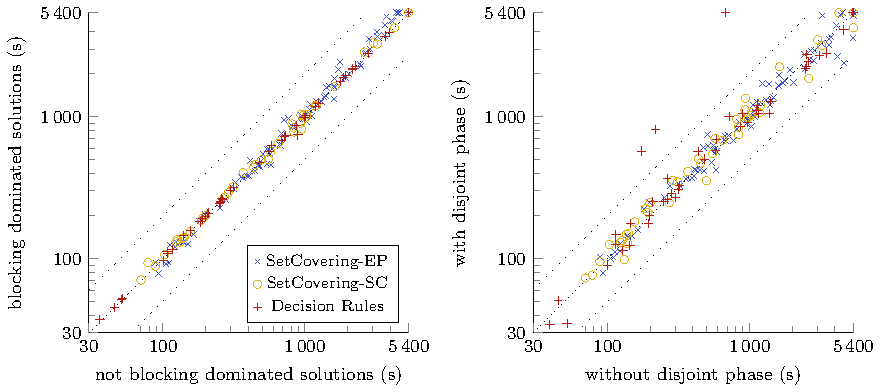
\includegraphics{all-datasets-chosen-refinements-2.pdf}
    \caption{Instance runtime comparisons for the two refinements blocking dominated solutions (left) and disjoint core extraction (right). \TODO{data not final}}\label{fig:refinements-2}
\end{figure}